\documentclass[../analisi-dei-requisiti.tex]{subfiles}

\begin{document}
La presente sezione ha lo scopo di descrivere in maniera dettagliata, attraverso il linguaggio \glossario{UML}, le funzionalità offerte da \glossario{Stalker}.

\subsection{Attori dei casi d'uso}%
\label{sub:attori_casi_duso}

\subsubsection{Applicazione mobile}%
\label{subs:mobile_app}

\begin{figure}[H]
  \centering
  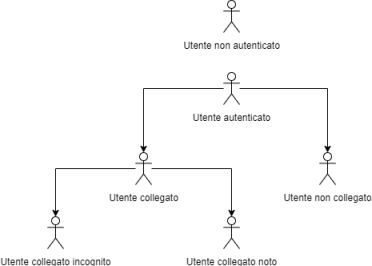
\includegraphics[width=100mm]{app_users.png}
  \caption{Utenti applicazione mobile}%
  \label{fig:usersapp}
\end{figure}

Un utente che accede per la prima volta all'applicazione mobile non è autenticato, quindi per accedere al sistema di Stalker inserisce le
credenziali per diventare un utente autenticato.
Successivamente a questo passaggio, l'utente può essere non collegato se non ha provveduto a collegarsi ad alcuna organizzazione, in caso contrario
è un utente autenticato che, in base all'organizzazione alla quale è collegato, può essere noto (con annessa autenticazione LDAP) oppure incognito.

\subsubsection{Web application}%
\label{subs:web_application}

\begin{figure}[H]
  \centering
  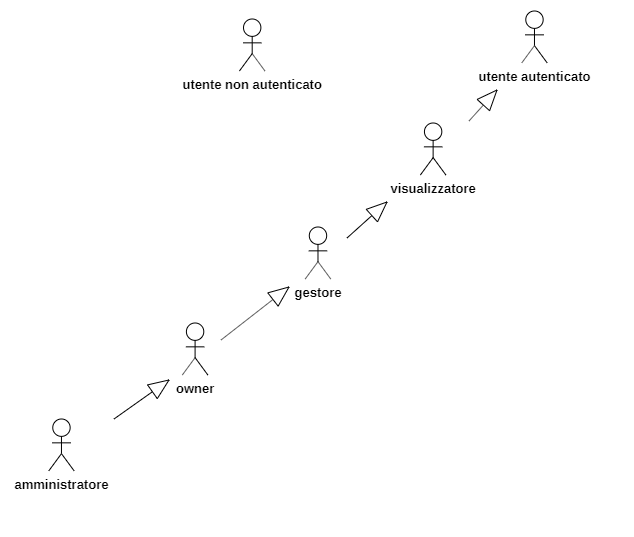
\includegraphics[width=100mm]{web_users.png}
  \caption{Utenti web application}%
  \label{fig:usersweb}
\end{figure}

Un utente che accede per la prima volta alla web application non è autenticato, quindi per accedere alla zona amministrativa di Stalker inserisce le
credenziali per diventare un utente autenticato.
Successivamente a questo passaggio, in base al tipo di privilegi l'utente può essere:
\begin{description}
  \item[visualizzatore]: visualizza determinate organizzazioni e i relativi luoghi, non ha permessi di modifica;
  \item[gestore]: gestisce i luoghi di una o più organizzazioni;
  \item[owner]: crea una o più organizzazioni, identificando i suoi gestori e visualizzatori.
\end{description}
L'amministratore assume tutti i privilegi che il sistema può offrire, gestendo tutte le organizzazioni e i relativi owner, gestori e visualizzatori.

\end{document}
